\documentclass[a4paper,spanish,12pt]{article}
\usepackage[spanish]{babel}
\usepackage[utf8]{inputenc}
\usepackage[pdftex]{graphicx}
\usepackage{vmargin}
\usepackage{float}
\usepackage{lastpage}
\usepackage{caratula}
\usepackage{url}
\usepackage{listings}
\usepackage{multirow}
%\usepackage{textcomp}
\usepackage{gensymb}
\usepackage{hyperref}
\usepackage[all]{hypcap}
\usepackage{array,booktabs}

\newcommand*{\fullref}[1]{\hyperref[{#1}]{\nameref*{#1} (\autoref*{#1})}} % One single link

%\hypersetup{
%    colorlinks,
%    citecolor=black,
%    filecolor=black,
%    linkcolor=black,
%    urlcolor=black
%}

%%%%%%%%%%%%%%%%%%%%%%%%%%%%%%%%%%%%%%%%%%%%%%%%%%%%%%%%%%%%%%%%%%%%%%%%%%%%%%%%
% Para que las imagenes queden en donde esta el comando poner esto en el       %
% preambulo y usar los flags de posicion htp o htpb                            %
%%%%%%%%%%%%%%%%%%%%%%%%%%%%%%%%%%%%%%%%%%%%%%%%%%%%%%%%%%%%%%%%%%%%%%%%%%%%%%%%
%
% Alter some LaTeX defaults for better treatment of figures:
% See p.105 of "TeX Unbound" for suggested values.
% See pp. 199-200 of Lamport's "LaTeX" book for details.
%   General parameters, for ALL pages:
\renewcommand{\topfraction}{0.9}	% max fraction of floats at top
\renewcommand{\bottomfraction}{0.8}	% max fraction of floats at bottom
%   Parameters for TEXT pages (not float pages):
\setcounter{topnumber}{2}
\setcounter{bottomnumber}{2}
\setcounter{totalnumber}{4}     % 2 may work better
\setcounter{dbltopnumber}{2}    % for 2-column pages
\renewcommand{\dbltopfraction}{0.9}	% fit big float above 2-col. text
\renewcommand{\textfraction}{0.07}	% allow minimal text w. figs
%   Parameters for FLOAT pages (not text pages):
\renewcommand{\floatpagefraction}{0.7}	% require fuller float pages
% N.B.: floatpagefraction MUST be less than topfraction !!
\renewcommand{\dblfloatpagefraction}{0.7}	% require fuller float pages

%%%%%%%%%%%%%%%%%%%%%%%%%%%%%%%%%%%%%%%%%
% ECO Para jugar con el footer. 		%
\usepackage{fancyhdr}					%
%%%%%%%%%%%%%%%%%%%%%%%%%%%%%%%%%%%%%%%%%


%%\usepackage{hyphenat}
%%\exhyphenpenalty=10000
%%\hyphenpenalty=10000
\setmarginsrb{10mm}% left margin
{15mm}% top margin
{15mm}% right margin
{10mm}% bottom margin
{0mm}{10mm}{0mm}{20mm}% we needed -- related to headers and footers

%%%%%%%%%
\pagestyle{fancy}
\fancyhf{}
\setlength\headheight{14.5pt}
\fancyhead[L, CE]{PedalerIA64 (Organización del Computador II)}
\fancyhead[R, CE]{Laporte Matías}
\fancyfoot[C]{ \thepage\ de \pageref{LastPage} }


%%%%%%%%%%

\begin{document}


%*************************************************************%
%                                                             %
% CARATULA                                                    %
%                                                             %
%*************************************************************%
    \materia{Organizaci\'on del Computador II}

    \titulo{Trabajo Práctico Final: PedalerIA64}
    \subtitulo{\textit{Informe}}

    \integrante{Laporte Matías}{686/09}{matiaslaporte@gmail.com}
    
    \maketitle
    
%*************************************************************%
%                                                             %
% INFORME                                                     %
%                                                             %
%*************************************************************%
\section{Introducción}
\label{sec:introduccion}

\indent El presente Trabajo Práctico consiste en el desarrollo de diversos efectos de audio que se pueden encontrar en softwares de edición en el contexto musical (Cubase, Reaktor, Audacity, etc.), así como también en pedaleras (de allí el nombre del programa) para el caso específico de una guitarra. 


\subsection{Proceso de desarrollo del TP}
\label{subsec:intro-desarrollo}
El proceso de desarrollo del \textbf{TP} consistió en realizar en primera instancia un rápido prototipado en Matlab/RStudio/Scilab (dependiendo de la disponibilidad de la computadora que se usara en ese momento; de ahora en más, me referiré a esos programas como \textbf{MRS}) de algoritmos y ecuaciones que se pudieran encontrar en Internet de diversos efectos. 

El uso de esos programas como primer acercamiento a un efecto facilitaba enormemente el trabajo, pues al utilizar un lenguaje de muy alto nivel se simplificaba el manejo de la lectura y escritura de los archivos, el espacio en memoria para los mismos, la manipulación de los datos (poder trabajar sobre un vector entero con una sola operación, por ejemplo), etc.\vspace{\baselineskip}

Una vez certificado que con ese algoritmo se consiguiera el efecto auditivo deseado, se pasó a desarrollarlo en \textbf{C}, siempre verificando que el resultado final de la señal coincidiera con el obtenido en \textbf{MRS}. Como utilizar el comando \textit{diff} de UNIX directamente sobre los archivos no siempre daba el resultado querido (aventuro a decir que por diferencias de aproximación entre \textbf{MRS} y \textbf{C}), se optó por otra metodología utilizando el programa \textbf{Audacity}, que se explicará en la sección \fullref{subsec:chequeo-diferencias}.\vspace{\baselineskip}

Obtenido el resultado deseado utilizando \textbf{C}, se pasó finalmente a programar el mismo algoritmo en \textbf{Assembler}, haciendo uso de las instrucciones que ofrece el conjunto de instrucciones SSE para manejar múltiples datos con una única instrucción (SIMD). Se utilizaron instrucciones incluidas hasta la extensión SSE4 (en particular por \textit{PTEST}, y \textit{ROUNDPS}/\textit{ROUNDSS}). 
Luego de obtener en \textbf{Assembler} un código que parecía aceptable (es decir, que no terminara abruptamente con un segfault), se comenzó con un proceso iterativo de corrección, mediante la comparación del archivo de audio obtenido con el de \textbf{C}, utilizando \textbf{Audacity} como se mencionó previamente. Las diferencias entre ambos muchas veces provenían de casos bordes; los problemas encontrados a lo largo del desarrollo del TP se tratarán en la sección \fullref{subsec:desarrollo-problemas}.\vspace{\baselineskip}

El objeto de la programación en \textbf{C} además de Assembler, si bien implica el ''doble'' de trabajo, se debe a dos puntos en particular. En primer medida, era una buena manera de poder bajar el nivel del código original en \textbf{MRS}, despojándolo de las bondades que dichas herramientas ofrecen. Por otro lado, tener el código en \textbf{C} sirve también para comparar la mejora de rendimiento con el uso de las instrucciones SIMD. \vspace{\baselineskip}

Para calcular el rendimiento en ambos lenguajes se utilizó la librería \textit{tiempo.h} utilizada por la cátedra en el \textbf{TP N\degree 2} del 1er. Cuatrimestre de 2011. Cuando los resultados con la misma no eran satisfactorios (p.ej., \textbf{Assembler} era más lento que \textbf{C}), se procedió a utilizar una herramienta de profiling (\textbf{callgrind} en conjunto con \textbf{KCacheGrind}, se hablará de ellas más adelante) para poder identificar dónde exactamente estaban las secciones lentas del código en \textbf{Assembler}, y poder tomar medidas para resolverlo. De los casos puntuales donde se utilizó esto se hablará en las secciones \fullref{sec:desarrollo}, \fullref{sec:resultados} y \fullref{sec:analisis}.\vspace{\baselineskip}

Se desarrolló también una rudimentaria interfaz gráfica para tratar de evitar la utilización de la línea de comandos (en particular por la cantidad de argumentos que hay que manipular para los diversos efectos) y que la utilización del programa sea más amigable. Se hablará de ella en la sección \fullref{subsec:gui}.
 

\newpage
\subsection{Audio}
\label{subsec:intro-audio}

\begin{figure}[H]
    \centering
    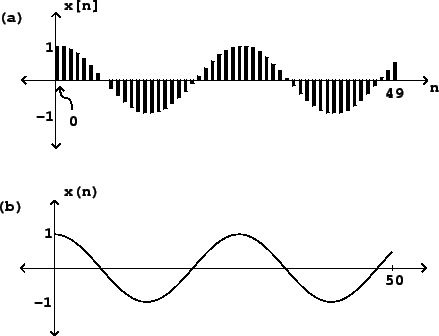
\includegraphics[scale=0.6]{imagenes/signals.png}
    \caption{Señales de audio}
    \label{fig:signals}
\end{figure}

Simplificándolo extremamente, una señal de audio (\textbf{(b)} en la figura \ref{fig:signals}) es una representación del sonido, que puede ser visualizado como una curva continua (en el caso analógico, sus valores representan voltaje eléctrico) en función del tiempo. Al digitalizar una señal, se discretiza la curva (\textbf{(a)} en la figura \ref{fig:signals}) tomando valores cada cierta cantidad de tiempo, lo que da lugar a la \textit{frecuencia de muestreo} (\textbf{sampling rate}, expresada como cantidad de muestras por segundo, unidad \textbf{Hz}). A la vez, cada uno de esos valores no puede ser expresado con precisión infinita, sino que al pasar al dominio digital, debe poder ser representado con una cantidad específica de bits, lo que origina la \textit{tasa de bits} (\textbf{bit rate}, \textit{resolución} de una señal de audio). \vspace{\baselineskip}

El formato de audio elegido para el \textbf{TP} es WAV \footnote{Más información aquí: \\ \url{http://stackoverflow.com/questions/13039846/what-do-the-bytes-in-a-wav-file-represent}}, por ser uno de los más simples para manipular. Los datos correspondientes al audio no están comprimidos, por lo que es posible realizar directamente sobre ellos las operaciones necesarias para aplicar los diversos efectos. En caso de que un archivo sea \textbf{stereo}, la información va intercalada (una muestra del canal izquierdo, otra del derecho, la siguiente del izquierdo, etc.).\vspace{\baselineskip}

La librería utilizada para el manejo de este tipo de archivo se verá en la sección \fullref{subsec:libsndfile}.\vspace{\baselineskip}

\fbox{\begin{minipage}{42em}
\underline{Nota}: por recomendación del profesor durante la presentación del proyecto de \textbf{TP}, en el archivo de audio final obtenido luego de la aplicación de alguno de los efectos, la \textit{señal seca} (\textit{dry sound/dry signal}, sin efecto) va por un canal, y la \textit{señal húmeda} (\textit{wet sound/wet signal}) por el otro. De este modo, se puede apreciar con mayor claridad el efecto en cuestión. 

\ \ \ \ Esto implica que todos los archivos de salida tendrán dos canales (\textbf{stereo}), a pesar de que el archivo de entrada pudiera haber tenido un único canal. En el caso de archivos de entrada con dos canales, se realiza un promedio de ambos (aunque esto sólo es válido en archivos stereo que mandan el mismo audio por los canales), y sobre ese nuevo ``canal'' se aplica el efecto correspondiente.
\end{minipage}} 
\label{output-stereo}
\newpage
\subsection{Herramientas externas utilizadas}
\label{subsec:herramientas}
Además de los ya mencionados \textbf{Matlab}, \textbf{RStudio}, y \textbf{Scilab}, se utilizaron las siguientas herramientas desarrolladas por terceros.

\subsubsection{libsndfile}
\label{subsec:libsndfile}
\textbf{libsndfile} es una librería de código abierto desarrollada en \textbf{C} para leer y escribir archivos de audio. Trabaja con el formato WAV, entre otros, por lo que se adaptaba a las necesidades del \textbf{TP}. La API puede consultarse aquí \footnote{\url{http://www.mega-nerd.com/libsndfile/api.html}}.\vspace{\baselineskip}

Una ventaja de la librería es que hace un pasaje de integer (tipo de datos utilizado en el formato WAV) a float, que es el tipo de datos utilizado para el \textbf{TP} \footnote{Originalmente se pensaba utilizar double, pero por recomendación del profesor se decidió pasar a float para poder procesar más datos}. Por otro lado, al leer un archivo utiliza una estructura propia llamada SF\_INFO, que incluye datos importantes del mismo (cantidad de canales, de muestras, entre otros), y que son necesarios en algunas porciones del \textbf{TP} por diversos motivos.

\subsubsection{Audacity}
\label{subsec:audacity}
\textbf{Audacity} es un editor multiplataforma de audio digital de código abierto y que en el \textbf{TP} se utilizó para realizar las comparaciones entre los archivos finales obtenidos de los diferentes efectos para cada lenguaje. De este modo, al no encontrar diferencias entre las señales de dos archivos diferentes, se podía corroborar que el algoritmo coincide con el efecto a aplicar.

\subsubsection{PyQt}
Para desarrollar la interfaz gráfica del TP, se utilizó PyQt5 (\textit{versión 5.2.1}), que provee bindings de Python (\textit{versión 3.x}) para el framework QT (\textit{versión 5.2.1}). Se verán los paquetes que será necesario instalar para usar la GUI en la sección \ref{subsec:instalar}

\subsubsection{Valgrind, KDbg, Callgrind, KCacheGrind}
Todas las herramientas mencionadas en el título fueron utilizadas para el debug del \textbf{TP}.

\subsubsection*{Valgrind}
\textbf{Valgrind} fue utilizado para saber cómo era el manejo de memoria del programa. En el caso de que el programa terminara repentinamente debido a algún \textit{segmentation fault}, mediante \textbf{Valgrind} se podía saber en qué línea del código ocurría, pasando entonces a ver cuál fue el acceso erróneo viendo los valores de los registros con \textbf{Kdbg}. 

\subsubsection*{KDbg}
Si bien en la materia se recomendaba utilizar DDD, a mi parecer tenía una interfaz bastante anticuada, y \textit{crasheaba} mucho; por esa razón se buscó una alternativa, y \textbf{Kdbg} resultó ser una opción más que adecuada para mis requerimientos, más estable y más amigable en cuanto a UI.

\subsubsection*{Callgrind}
Cuando había dudas con respecto a la performance del código en \textbf{Assembler} al compararlo con \textbf{C}, se buscó información sobre herramientas para profiling. Es posible utilizar \textbf{Valgrind} con una serie de argumentos especiales (\textit{--tool=callgrind --dump-instr=yes --collect-jumps=yes}) que devuelven un archivo de nombre callgrind.out.XXXXX (siendo XXXXX el número del proceso corrido) donde se encuentra toda la información sobre los llamados a instrucciones y dónde se pierde más tiempo en la ejecución de un programa.

\subsubsection*{KCacheGrind}
Para visualizar el archivo anterior, se utiliza KCacheGrind, que muestra toda la información de manera completamente intuitiva, y que permite identificar rápidamente dónde están los cuellos de botella del programa. Se verán los resultados obtenidos con el programa en la sección \ref{desarrolloponele}. 


\newpage
\subsection{Uso TP} 
\subsubsection{Paquetes a instalar}
\label{subsec:instalar}
Para esta sección, se instaló la distribución Linux Mint 17.1 (basada en Ubuntu) en una máquina virtual, de modo de poder saber qué es necesario instalar en un sistema desde 0 para poder correr el \textbf{TP}.

\subsubsection*{Compilar TP}
Para poder compilar el \textbf{TP} mediante el comando \textit{Make}, se necesitan los paquetes: 
\begin{itemize}
 \item \textbf{libsndfile1-dev} (librería libsndfile)
 \item \textbf{build-essential} (librería stdio.h)
 \item \textbf{nasm}
\end{itemize}

\subsubsection*{Interfaz gráfica}
Para poder ejecutar la interfaz gráfica:
\begin{itemize}
 \item \textbf{python3}
 \item \textbf{python3-pyqt5} (bindings de Qt para python3)
 \item \textbf{python3-pyqt5.qtmultimedia} (para poder reproducir archivos de audio desde la GUI)
\end{itemize}

\subsubsection*{Debug}
Para las herramientas de debug, es necesario instalar:
\begin{itemize}
 \item \textbf{valgrind}
 \item \textbf{kdbg}
 \item \textbf{kcachegrind}
 \item \textbf{graphviz libgraphviz-perl} (sólo para poder ver el Call Graph en KCacheGrind)
\end{itemize}

\subsubsection*{Comparación visual señales de audio}
Si se desea realizar la comparación visual de las señales de audio explicada en la sección \ref{subsec:chequeo-diferencias}, será necesario instalar el siguiente paquete:
\begin{itemize}
 \item \textbf{audacity}
\end{itemize}
\newpage
\subsubsection{Linea comandos}
\label{subsec:cli}
Una vez compilado el \textbf{TP} (mediante el comando \textit{make}, pues el archivo Makefile se encuentra incluido), se puede ver la ayuda del programa ejecutando únicamente \textit{./main}. Por razones de completitud, se explica aquí también cómo utilizar el programa. \vspace{\baselineskip}

La estructura para aplicar un efecto a un archivo de audio es la siguiente:

\lstset{language=bash}
\begin{lstlisting}[frame=single]
./main INFILE OUTFILE EFFECT ARGS
\end{lstlisting}

\begin{itemize}
 \item \textbf{INFILE} es el archivo de audio de entrada, siempre en formato WAV.
 \item \textbf{OUTFILE} es el nombre deseado del archivo de salida, con extensión .WAV.
 \item \textbf{EFFECT} es un guión, seguido del caracter asociado al efecto a aplicar.
 \item \textbf{ARGS} son los argumentos dependientes del efecto definido en \textbf{EFFECT}.
\end{itemize}

La lista de los efectos y los rangos de los argumentos correspondientes (los mismos se explicarán en la sección \ref{sec:desarrollo} de Desarrollo de cada efecto) se pueden consultar en la siguiente tabla:\vspace{\baselineskip}

\begin{table}[H]
\centering
\begin{tabular}{|c|c|c|c|l|l|c|c|l|c|l|c|c|l|l|}
\hline
\multirow{2}{*}{{\bf Nombre}} & \multicolumn{2}{c|}{{\bf Caracter}} & \multicolumn{12}{c|}{\multirow{2}{*}{{\bf Argumentos}}}                                                                                                                                                                                                                                                                                                       \\ \cline{2-3}
                              & {\bf ASM}         & {\bf C}         & \multicolumn{12}{c|}{}                                                                                                                                                                                                                                                                                                                                        \\ \hline
Copiar                        & C                 & c               & \multicolumn{12}{c|}{Ninguno}                                                                                                                                                                                                                                                                                                                                 \\ \hline
Delay                         & D                 & d               & \multicolumn{6}{c|}{\begin{tabular}[c]{@{}c@{}}\underline{Delay}:\\ 0.0-5.0 segundos\end{tabular}}                                                                                & \multicolumn{6}{c|}{\begin{tabular}[c]{@{}c@{}}\underline{Decay}: \\ 0.00-1.00\end{tabular}}                                                                                                      \\ \hline
Flanger                       & F                 & f               & \multicolumn{4}{c|}{\begin{tabular}[c]{@{}c@{}}\underline{Delay}: \\ 0-15 milisegundos\end{tabular}}                   & \multicolumn{4}{c|}{\begin{tabular}[c]{@{}c@{}}\underline{Rate}: \\ 0.1-5.0 hertz\end{tabular}}                                   & \multicolumn{4}{c|}{\begin{tabular}[c]{@{}c@{}}Amp: \\ 0.65-0.75\end{tabular}}                                           \\ \hline
Vibrato                       & V                 & v               & \multicolumn{6}{c|}{\begin{tabular}[c]{@{}c@{}}\underline{Depth}: \\ 0-3 milisegundos\end{tabular}}                                                                               & \multicolumn{6}{c|}{\begin{tabular}[c]{@{}c@{}}\underline{Mod}: \\ 0.1-5.0 hertz\end{tabular}}                                                                                                    \\ \hline
Bitcrusher                    & B                 & b               & \multicolumn{6}{c|}{\begin{tabular}[c]{@{}c@{}}\underline{Bits}:\\ 1-16\end{tabular}}                                                                                             & \multicolumn{6}{c|}{\begin{tabular}[c]{@{}c@{}}\underline{Bitrate}: \\ 1-44100 hertz\end{tabular}}                                                                                                \\ \hline
Wah Wah                       & W                 & w               & \multicolumn{3}{c|}{\begin{tabular}[c]{@{}c@{}}\underline{Damp}:\\ 0.1-1.0\end{tabular}} & \multicolumn{3}{c|}{\begin{tabular}[c]{@{}c@{}}\underline{MinFreq}:\\ 400-1000 hertz\end{tabular}} & \multicolumn{3}{c|}{\begin{tabular}[c]{@{}c@{}}\underline{MaxFreq}:\\ 2500-3500 hertz\end{tabular}} & \multicolumn{3}{c|}{\begin{tabular}[c]{@{}c@{}}\underline{WahWah Freq}:\\ 1000-3000 hertz\end{tabular}} \\ \hline
\end{tabular}
\caption{Lista de comandos}
\label{tab:efectos}
\end{table}
\newpage
\subsubsection{GUI}
\label{subsec:gui}
La GUI intenta ser una manera más intuitiva de ejecutar el programa, sin necesidad de tener que ingresar todos los argumentos a mano. Se ejecuta (estando en la carpeta \textbf{src}) mediante el siguiente comando:

\begin{center}\textit{python3 gui/main.py}\end{center}\vspace{\baselineskip}

\begin{figure}[H]
    \centering
    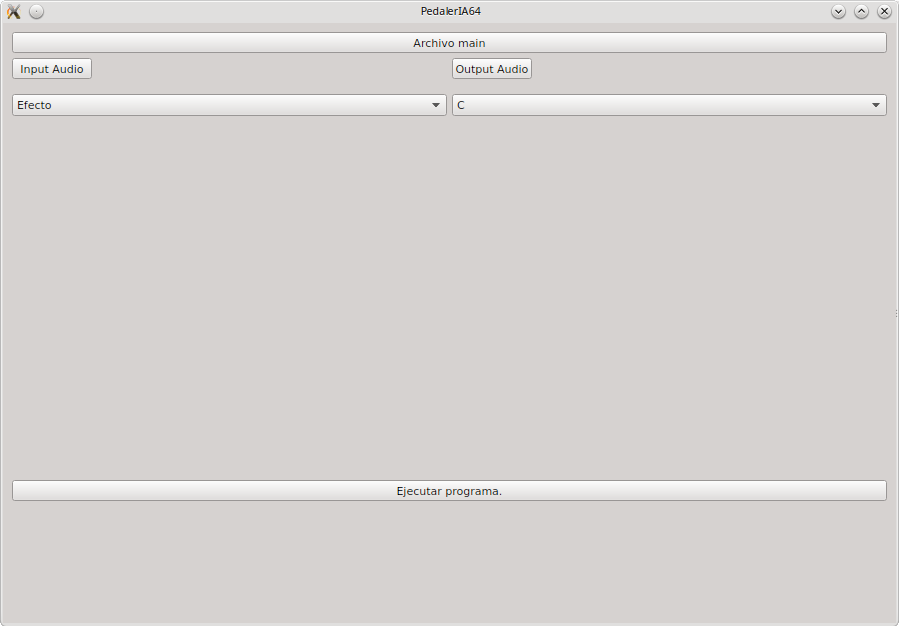
\includegraphics[scale=0.68]{imagenes/gui.png}
    \caption{GUI}
    \label{fig:gui}
\end{figure}

La GUI limpia se ve en la figura \ref{fig:gui}. Es necesario seleccionar dónde se encuentra el archivo \textbf{main}, el archivo de entrada sobre el cual se quiere aplicar el efecto, cuál es el nombre deseado del archivo de salida (se lo colocará en la misma carpeta donde se encuentra \textbf{main}) y, finalmente, el efecto a aplicar junto con sus argumentos.\vspace{\baselineskip}

La GUI con todos los argumentos completados, y luego de seleccionar el botón ``ejecutar programa'' se ve como en la figura \ref{fig:gui-complete}.\vspace{\baselineskip}

\begin{figure}[H]
    \centering
    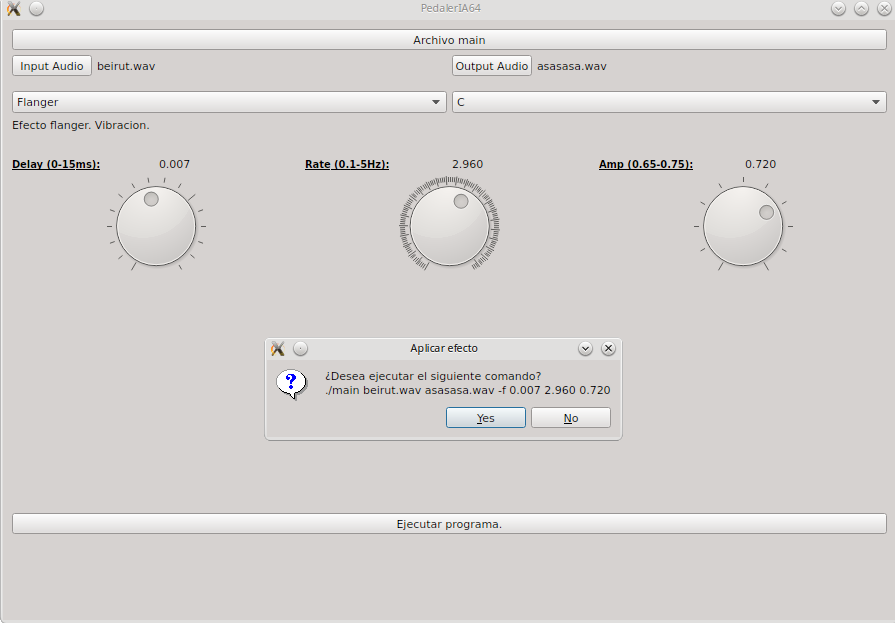
\includegraphics[scale=0.68]{imagenes/gui-complete.png}
    \caption{GUI con todas las opciones seleccionadas}
    \label{fig:gui-complete}
\end{figure}

\begin{center}
\fbox{\begin{minipage}{42em}
\underline{Nota}: En el popup para confirmar si el comando es el correcto, el mismo no representa exactamente lo que se ejecuta, pues faltan los paths hacia cada archivo. Para que no quede un texto largo e incomprensible en el popup, se decidió poner únicamente los nombres de los MAIN, INFILE y OUTFILE, aún cuando los primeros dos podrían no compartir carpeta (OUTFILE siempre está en la misma carpeta que MAIN).
\end{minipage}}
\end{center}\vspace{\baselineskip}

Al poner ``Yes'', la interfaz ejecutará el comando y, en caso de que todo haya salido correctamente, ofrecerá dos botones para poder reproducir el audio de entrada, el de salida, y comparar, como se puede ver en la figura \ref{fig:gui-play-buttons}.

\begin{figure}[H]
    \centering
    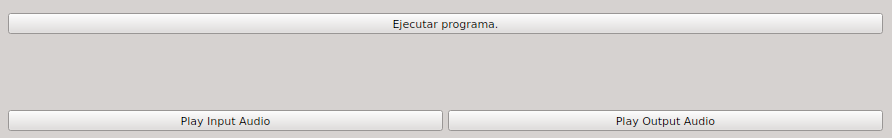
\includegraphics[scale=0.68]{imagenes/gui-play-buttons.png}
    \caption{Botones de reproducción}
    \label{fig:gui-play-buttons}
\end{figure}

En caso de que falle, se dará noticia de eso, pero no se manejará ni mostrará el error (se recomienda ejecutar el mismo comando que hubiera ejecutado la GUI en la CLI para ver qué pasó; de todos modos, es posible ver el error en la terminal desde donde se haya corrido Python).

En caso de que falte completar alguna opción, al hacer click en ``Ejecutar programa'' aparecerá un popup informando cuál es la opción que falta. 

\newpage
\subsubsection{Chequeo de diferencias con Audacity}
\label{subsec:chequeo-diferencias}
Para poder verificar si hay diferencias entre dos archivos de audio en Audacity, es necesario proceder del siguiente modo. Con el programa abierto, se arrastran los dos archivos hacia la ventana del mismo para que sean importados automáticamente (si es la primera vez, se va a preguntar si se quiere trabajar sobre los mismos archivos, o sobre una copia temporal de los mismos; por seguridad, se recomienda elegir esta última opción, y que el programa la recuerde).\vspace{\baselineskip}

Como ambos archivos son ``de salida'' (para nuestro programa), serán los dos stereo. Es necesario separar los canales de cada uno de los archivos, para compararlos entre sí. Hacer click sobre la flecha al lado del nombre del archivo, y clickear en ``Split Stereo to Mono'' (o presionar la tecla \textbf{n}); ver figura \ref{fig:audacity-split-stereo}.


\begin{figure}[H]
    \centering
    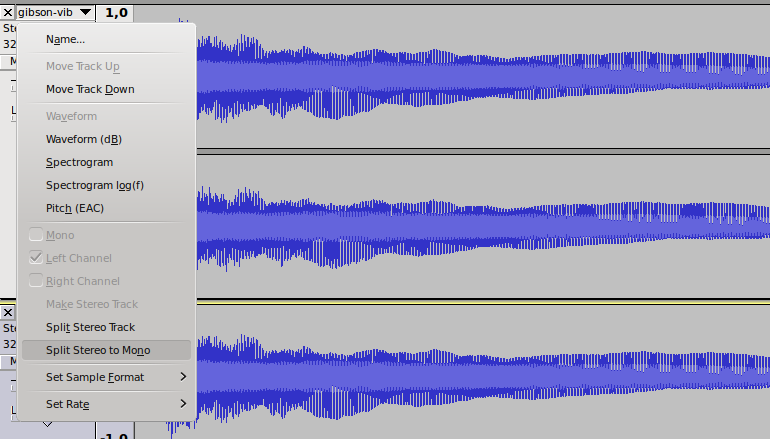
\includegraphics[scale=0.70]{imagenes/audacity-split-stereo.png}
    \caption{Convertir Stereo a canales Mono}
    \label{fig:audacity-split-stereo}
\end{figure}


Separados ya los canales de ambos archivos, seleccionar el canal izquierdo del primer archivo (aparecerá con un color diferente al resto), e ir al menú ``Effect'' (\textbf{Alt+c}), y elegir ``Invert''; ver figura \ref{fig:audacity-invert}.\vspace{\baselineskip}

\begin{figure}[H]
    \centering
    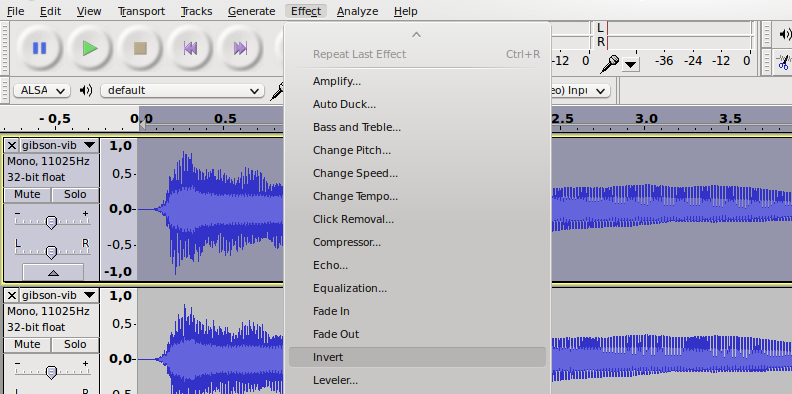
\includegraphics[scale=0.68]{imagenes/audacity-invert.png}
    \caption{Invertir canal}
    \label{fig:audacity-invert}
\end{figure}

Invertido, por ejemplo, el canal izquierdo del primer archivo, se selecciona dicho canal, junto con el izquierdo del segundo archivo (\textbf{shift+click} en los cuadrantes grises a la izquierda de cada señal). Con los dos canales correspondientes seleccionados, uno de ellos invertido, se va al menú ``Tracks'' (\textbf{Alt+t}), y se selecciona la opción ``Mix and Render'' (tecla \textbf{x}); ver figura \ref{fig:audacity-mix-and-render}.

\begin{figure}[H]
    \centering
    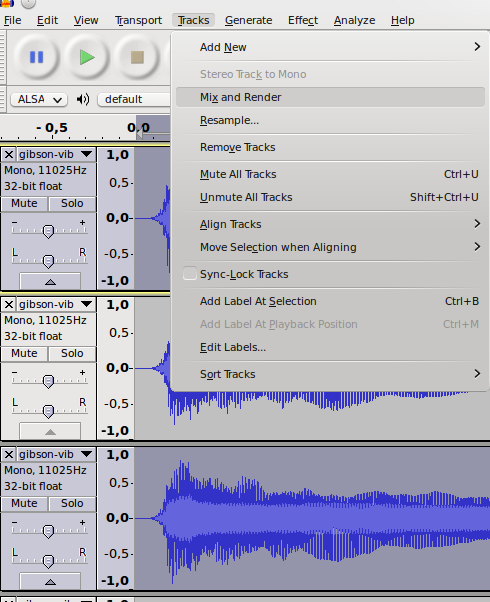
\includegraphics[scale=0.70]{imagenes/audacity-mix-and-render.png}
    \caption{Mix and render}
    \label{fig:audacity-mix-and-render}
\end{figure}

Los dos canales seleccionados que fueron mezclados, originalmente tenían la misma información. Al invertir uno de ellos, y mezclarlos entre sí, se produce una cancelación de la onda. Por lo tanto, si efectivamente contenían la misma información, debería verse el nuevo canal generado completamente vacío; ver figura \ref{fig:audacity-no-wave}. Durante el desarrollo del \textbf{TP}, esto a veces se consiguió y otras no, y las razones de ello se verán en las secciones correspondientes.

\begin{figure}[H]
    \centering
    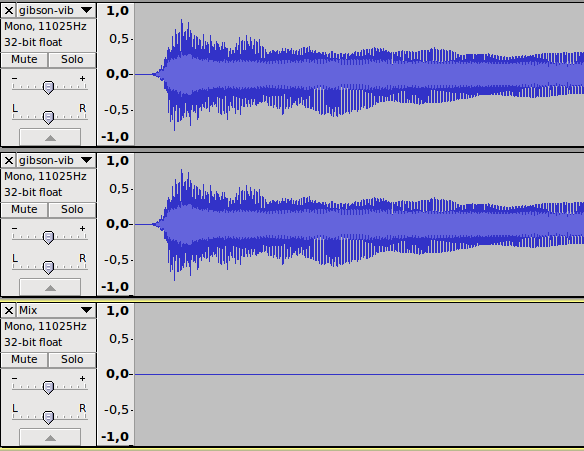
\includegraphics[scale=0.70]{imagenes/audacity-no-wave.png}
    \caption{Cancelación de la onda}
    \label{fig:audacity-no-wave}
\end{figure}

El canal izquierdo es la señal seca; repetir luego el mismo procedimiento con los dos canales derechos restantes. 


\newpage
\section{Desarrollo}
\label{sec:desarrollo}

\subsection{Estructura del código}
\label{subsec:desarrollo-estructura}
La carpeta correspondiente al código del \textbf{TP} (\textbf{src}) contiene 4 carpetas, y varios archivos. Las carpetas son las siguientes:
\begin{itemize}
  \item \textbf{gui}: contiene únicamente el archivo main.py, que es el que provee la interfaz gráfica para el \textbf{TP}.
  \item \textbf{inputExamples}: algunos archivos de audio en formato WAV como ejemplo de entrada.
  \item \textbf{outputExamples}: algunos archivos de audio en formato WAV como ejemplo de salida del programa. En sus nombres se encuentra expresado cuál fue el archivo de audio de entrada utilizado, cuál fue el efecto aplicado (y la versión, \textbf{C} o \textbf{Assembler}), y los valores de los argumentos de entrada.
  \item \textbf{libs}: incluye los archivos ssemathfun.h (sección \nameref{subsec:ssemath}) y tiempo.h (ver \ref{subsec:intro-desarrollo}).
\end{itemize}

Los archivos son los siguientes:

\begin{itemize}
 \item \textbf{main.c}: el archivo principal, que da nombre al ejecutable. Muestra la ayuda del programa, hace chequeo básico de errores en cuanto a los parámetros de entrada, crea punteros a los archivos de entrada y de salida, y llama al efecto correspondiente.
 \item \textbf{effects.h}: archivo donde se incluyen las librerías utilizadas, se declaran variables y constantes globales, y los encabezados de las funciones tanto en \textbf{C} como en \textbf{Assembler} (que serán de tipo \textit{extern}). Al final de este archivo se encuentra comentado el template básico (\fullref{subsec:desarrollo-comun}) con el código común que utilizan todos los efectos.
 \item \textbf{effects.c}: aquí se encuentran definidas todas las funciones auxiliares, y los efectos hechos en \textbf{C}.
 \item \textbf{effects\_asm.c}: el mismo contenido el anterior, pero donde se aplica un efecto o se realiza una operación en una función auxiliar, se llama a la función correspondiente en \textbf{Assembler}.
 \item \textbf{ARCHIVO.asm}: cada archivo con extensión .ASM corresponde al efecto o función auxiliar en cuestión.
 \item \textbf{Makefile}: archivo que permite compilar todo el \textbf{TP} mediante el comando \textit{make}.
\end{itemize}

\newpage
\subsection{Funciones auxiliares}
\label{subsec:desarrollo-auxiliares}

\subsubsection{Normalización}
\label{subsec:desarrollo-normalizacion}
Como se verá en la sección \fullref{subsec:desarrollo-problemas}, fue necesario desarrollar un algoritmo para normalizar un archivo de audio. Para esto se desarrollaron dos rutinas, una que busca la muestra de mayor valor absoluto en el archivo (\textbf{maxsamp\_right}), y otra que normaliza el  archivo completo en base a dicha muestra (\textbf{normalization\_right}).

Como la normalización sólo se realiza sobre un archivo al que le fue aplicado el efecto, sabemos que éste siempre va a ser stereo (\ref{output-stereo}) y, además, que la operación sólo será necesario hacerla sobre el canal derecho, que es el que tiene la señal húmeda (de allí el nombre \textbf{\_right}).

Se desarrollaron ambas rutinas tanto en ASM como en C, y la comparación de las versiones se verá en \fullref{subsec:resultados-normalization} y el análisis en \fullref{subsec:analisis-normalization}.

\subsubsection{Seno}
\label{subsec:desarrollo-seno}
En un principio, se intentó utilizar una librería para calcular el seno con instrucciones SIMD (\fullref{subsec:ssemath}) con bastante precisión; sin embargo, la pérdida de rendimiento al usar dicha librería de los algoritmos en ASM frente a los de C era muy notoria. Por esa razón, se recurrió a una solución \footnote{\url{http://forum.devmaster.net/t/fast-and-accurate-sine-cosine/9648/4}} para calcular el seno que realiza una aproximación mediante parábolas.

La rutina se encuentra en el archivo \textbf{sine.asm}, aunque el código para calcular el seno se terminó poniendo en cada lugar donde se necesitara (porque el cálculo de los argumentos era diferente para cada efecto, al igual que las operaciones posteriores a la obtención del seno).

\newpage
\subsection{Código común para los efecto}
\label{subsec:desarrollo-comun}

Todos los efectos tienen una parte común en su código, en lo que respecta a \textit{setteo} de variables, la creación de los buffers que serán utilizados, la lectura del archivo de entrada y escritura del archivo de salida. Esa parte común sigue más o menos la siguiente estructura.\vspace{\baselineskip}
El tamaño de los buffers depende de cada efecto en particular, pues no todos necesitan acceder en un ciclo a la misma cantidad de datos. Si bien se definió un tamaño ``común'' (BUFFERSIZE, definido en \textbf{effects.h}, de 8192), en algunos casos un efecto puede necesitar acceder a una cantidad de elementos que es función de alguno de los argumentos (en el caso de los efectos con delay, por ejemplo, donde se necesita que el tamaño del buffer sea múltiplo del argumento en cuestión).

\subsubsection{Pseudocódigo}

\lstset{literate={á}{{\'a}}1
        {ã}{{\~a}}1
        {é}{{\'e}}1
        {ó}{{\'o}}1
        {í}{{\'i}}1
        {ñ}{{\~n}}1
        {¡}{{!`}}1
        {¿}{{?`}}1
        {ú}{{\'u}}1
        {Í}{{\'I}}1
        {Ó}{{\'O}}1
        }
        
\begin{lstlisting}[frame=single]

Definición de variables para la creación de los buffers
	  (de entrada, de salida, y los necesarios para los efectos)

Crear los buffers necesarios con el tamaño adecuado

Definición de variables utilizadas para los efectos (no ocurre en todos).


Mientras haya datos por leer
    Leer archivo de entrada y guardar los datos en el buffer de entrada
    Recorrer el buffer de entrada
      Si el archivo es stereo, calcular promedio de los dos canales
    
      Contar cantidad de ciclos de reloj
	Aplicar operación sobre los datos de entrada
      Dejar de contar cantidad de ciclos de reloj
    
      Guardar el resultado en el buffer de salida
    Dejar de recorrer el buffer de entrada
    
    Guardar el buffer de salida en el archivo de salida
Dejar de leer datos

Liberar memoria utilizada por los buffers
\end{lstlisting}

\newpage
\subsection{Copy}
\label{subsec:desarrollo-copy}

\subsubsection{Descripción}
\label{subsec:desarrollo-copy-desc}

No es un efecto en sí, pero fue desarrollado como prueba de concepto para el preinforme, como método para verificar que se estuviera usando bien la API de libsndfile (\ref{subsec:libsndfile-api}), la convención de llamado de funciones de ASM desde C, entre otras cosas.

\begin{center}
\fbox{\begin{minipage}{32em}
\underline{Nota}: en el preinforme, este algoritmo utilizaba doubles en vez de floats.
\end{minipage}}
\end{center}

Los resultados de la comparación entre las versiones en \textbf{C} y \textbf{ASM} de este algoritmo se verán en la sección \fullref{subsec:resultados-copy}, y el análisis en \fullref{subsec:analisis-copy}.

\subsubsection{Pseudocódigo}
\label{subsec:desarrollo-copy-code}

No se adjunta el pseudocódigo para este algoritmo por no aportar nada, pues es literalmente grabar en el buffer de salida lo que contiene el buffer de entrada.

\subsubsection{Comando}
\label{subsec:desarrollo-copy-call}

\underline{\textbf{C}}:
\begin{center}
 \textit{./main INFILE OUTFILE -c}
\end{center}

\underline{\textbf{ASM}}:
\begin{center}
 \textit{./main INFILE OUTFILE -C}
\end{center}
\newpage
\subsection{Delay simple}
\label{subsec:desarrollo-delay}

\subsubsection{Descripción}
\label{subsec:desarrollo-delay-desc}

El delay simple es uno de los efectos más básicos en Audio DSP. Consiste simplemente en retrasar la entrada una cantidad arbitraria de segundos; se puede, también, aplicar un modificador para que la señal húmeda sea un porcentaje de la señal original (para que no suenen ambas con la misma intensidad).

A diferencia de otros efectos en los que se hace uso de una cantidad mínima (medida en milisegundos) para delay, aquí tiene una magnitud mayor, por lo que el archivo de salida tendrá una duración mayor que el de entrada. Esto ocasiona que cuando ya no quedan más datos para leer, se realice un ciclo más de escritura, donde se vierte la entrada obtenida en el último ciclo de lectura.

En este efecto, se calcula a cuántas muestras (\textbf{frames}) equivale el argumento de delay (que está en segundos), mediante el cálculo
\begin{center}$delayInFrames = ceil(delayInSec*inFileStr.samplerate)$.\end{center}

El tamaño de los buffers a usar (\textit{dataBuffIn}, \textit{dataBuffOut} y \textit{dataBuffEffect}) será el máximo entre \textit{delayInFrames} y el mayor múltiplo de dicho valor que sea menor que BUFFERSIZE (8192). \textit{dataBuffEffect} contiene siempre la entrada del ciclo anterior; de este modo, nos aseguramos que en cada ciclo de lecto/escritura se pueda acceder mediante \textit{dataBuffEffect} a lo que se leyó en el ciclo anterior, que pasó hace una cantidad \textit{delay} de segundos, que es lo que necesita el efecto.

\vspace{\baselineskip}

Los resultados de la comparación entre las versiones en \textbf{C} y \textbf{ASM} de este algoritmo se verán en la sección \fullref{subsec:resultados-delay}, y el análisis en \fullref{subsec:analisis-delay}.

\subsubsection{Pseudocódigo}
\label{subsec:desarrollo-delay-code}

\lstset{language=C}
\begin{lstlisting}[frame=single]
Argumentos: delay, decay
dataBuffOut.canalDerecho = dataBuffIn.muestraCicloAnterior * decay
dataBuffOut.canalIzquierdo = dataBuffIn.muestracicloActual
\end{lstlisting}

\subsubsection{Comando}
\label{subsec:desarrollo-delay-call}

\underline{\textbf{C}}:
\begin{center}
 \textit{./main INFILE OUTFILE -d delay decay}
\end{center}

\underline{\textbf{ASM}}:
\begin{center}
 \textit{./main INFILE OUTFILE -D delay decay}
\end{center}

\begin{itemize}
 \item \textit{delay}: argumento sin rango específico, pero por conveniencia se lo limitó en la GUI al rango [0.0, 5.0] segundos. Es la cantidad de segundos de retraso que se quiere tener en la señal húmeda.
 \item \textit{decay}: argumento con rango entre 0.00 y 1.00. Es el porcentaje de la amplitud de la señal seca que se quiere en la señal húmeda.
\end{itemize}

\newpage
\subsection{Flanger}
\label{subsec:desarrollo-flanger}

\subsubsection{Descripción}
\label{subsec:desarrollo-flanger-desc}

Flanger es un efecto que en sus orígenes se conseguía del siguiente modo. Se tenían dos cintas con el mismo material de audio, el original y una copia, y se mezclaban en un tercer canal. Este hecho ya generaba una pequeña diferencia de fase; pero además, durante la reproducción de la cinta duplicada, se presionaba sutilmente con el dedo el borde (\textit{flange}) de la bobina de la cinta, lo que afectaba la velocidad de reproducción y agregaba a la diferencia de fase una leve diferencia temporal, proununciado el efecto.

En el caso digital, se utiliza un \textbf{LFO} (\textit{low frequency oscillator}) para variar la velocidad de reproducción de la copia. El LFO se genera calculando el valor absoluto del seno de un valor que es función del índice de la muestra actual y del parámetro \textbf{rate} del efecto; este resultado parcial (que está entre 0 y 1, y es una onda que varía periódicamente según el índice de la muestra) se multiplica por el parámetro  \textbf{delay}; de este modo, se obtiene para el índice actual (señal original), cuál es la muestra anterior (de la señal duplicada) que se le debe sumar. Esta señal original no se añade en su totalidad, sino que se multiplica por el parámetro \textbf{amp} para atenuarla levemente.

\vspace{\baselineskip}

Los resultados de la comparación entre las versiones en \textbf{C} y \textbf{ASM} de este algoritmo se verán en la sección \fullref{subsec:resultados-flanger}, y el análisis en \fullref{subsec:analisis-flanger}.

\subsubsection{Pseudocódigo}
\label{subsec:desarrollo-flanger-code}

\lstset{language=C}
\begin{lstlisting}[frame=single]
Argumentos: delay, rate, amp
Para cada muestra
  arg_seno = 2*PI*indice_muestra * rate/archivoEntrada.samplerate
  seno_actual = | seno(arg_seno) |
  delay_actual = ceiling(seno_actual*delay)
  indice_copia = indice_muestra-delay_actual
  
  dataBuffOut.canalDerecho =  dataBuffIn.muestraCicloActual*amp + 
			      dataBuffIn.muestra_indice_copia*amp
  dataBuffOut.canalIzquierdo = dataBuffIn.muestraCicloActual
\end{lstlisting}

\subsubsection{Comando}
\label{subsec:desarrollo-flanger-call}

\underline{\textbf{C}}:
\begin{center}
 \textit{./main INFILE OUTFILE -f delay rate amp}
\end{center}

\underline{\textbf{ASM}}:
\begin{center}
 \textit{./main INFILE OUTFILE -F delay rate amp}
\end{center}

\begin{itemize}
 \item \textit{delay}: argumento con rango entre 0.000-0.015s. Es el delay máximo que puede tener la muestra duplicada.
 \item \textit{rate}: argumento con rango entre 0.1-5Hz. Es la frecuencia del LFO.
 \item \textit{amp}: argumento con rango entre 0.65 y 0.75. Según bibliografía consultada \footnote{\cite[p.~77]{zolzer11}}, el valor es 0.7, pero para hacerlo variable se eligió el rango 0.65-0.75. Es el porcentaje de la amplitud de la señal duplicada.
\end{itemize}
\newpage
\subsection{Vibrato}
\label{subsec:desarrollo-vibrato}

\subsubsection{Descripción}
\label{subsec:desarrollo-vibrato-desc}

Vibrato es un efecto que consiste en \textit{la variación periódica de la frecuencia de un sonido}\footnote{\url{https://es.wikipedia.org/wiki/Vibrato}}. Esta variación puede conseguirse utilizando un \textbf{LFO}, como en el efecto anterior, pero en este caso lo que oscilará es la frecuencia (\textbf{pitch}) del sonido, y no el delay de la señal (que además, en el vibrato, el delay toma un valor mucho menor, 0-3ms). 

Para este efecto, se utilizó un buffer circular (\textit{dataBuffEffect}). El \textbf{LFO} toma los mismos parámetros que en \fullref{subsec:desarrollo-flanger}, el argumento \textbf{mod} del efecto (que simboliza la frecuencia de modulación) y el índice de la muestra actual. La parte entera de este resultado es el índice de la muestra que se utiliza en la señal húmeda, mientras que la parte fraccionaria se usa para realizar una interpolación entre la mencionada muestra y la anterior.

Al igual que para el caso del \fullref{subsec:desarrollo-flanger}, la rutina en \textbf{ASM} se encuentra dividida en dos archivos, \textbf{vibrato\_index\_calc.asm} y \textbf{vibrato.asm}.

\vspace{\baselineskip}

Los resultados de la comparación entre las versiones en \textbf{C} y \textbf{ASM} de este algoritmo se verán en la sección \fullref{subsec:resultados-vibrato}, y el análisis en \fullref{subsec:analisis-vibrato}.

\subsubsection{Pseudocódigo}
\label{subsec:desarrollo-vibrato-code}

\lstset{language=C}
\begin{lstlisting}[frame=single]
Argumentos = mod, depth
depth = redondear(depth*archivoEntrada.samplerate)
delay = depth
mod = mod/archivoEntrada.samplerate
Para cada muestra
  mod_actual = sen(mod*2*PI*indice_actual)
  tap = 1+delay+depth*mod_actual
  indice_muestra_humeda = floor(tap)
  frac = tap - indice_muestra_humeda

  dataBuffOut.canalDerecho =  dataBuffIn.muestra_humeda*frac + 
			      dataBuffIn.(muestra_humeda-1)*(1-frac)
  dataBuffOut.canalIzquierdo = dataBuffIn.muestraCicloActual
\end{lstlisting}

\subsubsection{Comando}
\label{subsec:desarrollo-vibrato-call}

\underline{\textbf{C}}:
\begin{center}
 \textit{./main INFILE OUTFILE -v depth mod}
\end{center}

\underline{\textbf{ASM}}:
\begin{center}
 \textit{./main INFILE OUTFILE -V depth mod}
\end{center}

\begin{itemize}
 \item \textit{depth}: argumento con rango entre 0.000 y 0.003s. Es el delay de la señal de entrada.
 \item \textit{mod}: argumento con rango entre 0.10 y 5.00Hz. Es la frecuencia de modulación del efecto.
\end{itemize}
 

\newpage
\subsection{Bitcrusher}
\label{subsec:desarrollo-bitcrusher}

\subsubsection{Descripción}
\label{subsec:desarrollo-bitcrusher-desc}
En la sección \fullref{subsec:intro-audio} se habló sobre dos medidas de audio digital que son quienes determinan la \textit{calidad} del sonido: la frecuencia de muestreo (\textit{sampling rate}) y la resolución de la muestra (\textit{bit rate}). El efecto \textbf{bitcrusher} provoca una distorsión de la señal original, reduciendo tanto el muestreo (se toma en la señal húmeda una de cada cierta cantidad de muestras de la señal original, \textbf{downsampling}) como la cantidad de bits con la que se puede expresar cada muestra.

Los resultados de este efecto muchas veces hacen recordar a la música de los primeros juegos de consola (también conocidas como \textbf{chiptunes}), pues eran generadas con chips de 8 bits.

En la siguiente imagen, puede apreciarse cómo el efecto distorsiona la señal original (onda superior).

\begin{figure}[H]
    \centering
    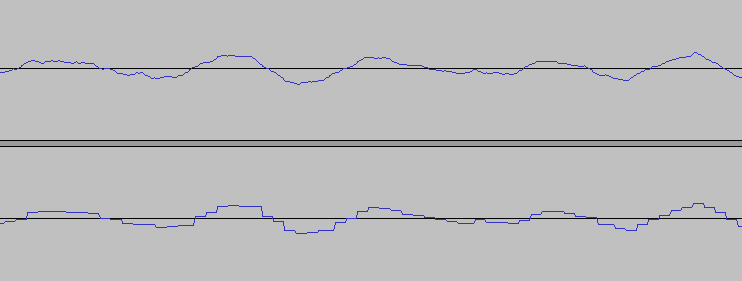
\includegraphics[scale=0.6]{imagenes/bitcrusher-signal.png}
    \caption{Señal superior: original. Señal inferior: al aplicar el efecto.}
    \label{fig:bitcrusher-signals}
\end{figure}


\vspace{\baselineskip}

Los resultados de la comparación entre las versiones en \textbf{C} y \textbf{ASM} de este algoritmo se verán en la sección \fullref{subsec:resultados-bitcrusher}, y el análisis en \fullref{sec:analisis}.

\subsubsection{Pseudocódigo}
\label{subsec:desarrollo-bitcrusher-code}

\lstset{language=C}
\begin{lstlisting}[frame=single]
??
\end{lstlisting}

\subsubsection{Comando}
\label{subsec:desarrollo-bitcrusher-call}

\underline{\textbf{C}}:
\begin{center}
 \textit{./main INFILE OUTFILE -}
\end{center}

\underline{\textbf{ASM}}:
\begin{center}
 \textit{./main INFILE OUTFILE -}
\end{center}

\begin{itemize}
 \item \textit{bits}: argumento con rango entre 1 y 16. Es la cantidad de bits que se pueden utilizar para el valor de cada muestra.
 \item \textit{freq}: argumento con rango entre 2048 y 11025Hz. Es la frecuencia de sampleo de la señal húmeda.
\end{itemize}
 
 

\newpage
\subsection{WahWah}
\label{subsec:desarrollo-wahwah}

\subsubsection{Descripción}
\label{subsec:desarrollo-wahwah-desc}

WahWah es uno de los efectos más conocidos y fáciles de identificar, pues su nombre describe el sonido que genera. El efecto se genera con la aplicación de un filtro pasabanda (sólo deja pasar las frecuencias entre dos valores, mínimo y máximo, preestablecidos) que varía con el tiempo. El filtro pasabanda se implementó mediante un filtro de estado variable (que permite separar a la señal original \textit{x} en tres, debajo del pasa banda $y_{l}$, en el pasa banda $y_{b}$, y por arriba del pasa banda $y_{h}$), que sigue las siguientes ecuaciones:

\begin{center}
 $y_{l}(n) = F_{c} * y_{b}(n) + y_{l}(n-1) $ \\
 $y_{b}(n) = F_{c} * y_{h}(n) + y_{b}(n-1) $\\
 $y_{h}(n) = x(n) - y_{l}(n-1) - Q_{1} * y_{b}(n-1)$
\end{center}

$F_{c}$ es un valor que depende de las frecuencias de corte del filtro pasa banda (implementado con una onda triangular con los valores centrales de frecuencia), y $Q_{1}$ está relacionado con el argumento \textit{damp}, que especifica el tamaño de las bandas. La onda triangular es cíclica, tiene mínimo \textbf{minf} y máximo \textbf{maxf}, y en cada punto va creciendo/decreciendo en el valor \textbf{delta}. Para no guardar los valores de la onda triangular en un buffer, se generan puntualmente; primero se calcula para cada muestra si correspondería a un punto de un ciclo de crecimiento (``par'') o decrecimiento (``impar'') de la onda, y luego qué punto de ese ciclo es. Este valor es intermedio al cálculo final del $F_{c}$ que se ve en la ecuación de arriba.

En este efecto se dio la particularidad de que en algunos casos las operaciones \textit{saturaban} algunas muestras. Por esa razón se debió optar por la \fullref{subsec:desarrollo-normalizacion} del archivo, por razones que se explicarán en \fullref{subsec:desarrollo-problemas-normalizacion}, primero se tuvo que ``achicar'' el valor de las muestras, por lo que se les aplicó un modificador de 0.1 a la señal húmeda. Si bien esto aumenta el error numérico, fue la solución más convincente.


La rutina en \textbf{ASM} se encuentra dividida también en dos archivos, \textbf{wah\_wah\_index\_calc.asm} y \textbf{wah\_wah.asm}.

\vspace{\baselineskip}

Los resultados de la comparación entre las versiones en \textbf{C} y \textbf{ASM} de este algoritmo se verán en la sección \fullref{subsec:resultados-wahwah}, y el análisis en \fullref{subsec:analisis-wahwah}.

\subsubsection{Pseudocódigo}
\label{subsec:desarrollo-wahwah-code}

\lstset{language=C}
\begin{lstlisting}[frame=single]
Argumentos: damp, minFreq, maxFreq, wahWahFreq
q1 = 2*damp
delta = wahWahFreq/archivoEntrada.samplerate	
triangleWaveSize = floor((maxFreq-minFreq)/delta)+1

yh = yb = yl = 0

Para cada muestra
  cicloPar = (indice_muestra_actual/triangleWaveSize)%2 
  esteCiclo = (indice_muestra_actual) % triangleWaveSize + 1
  
  fc = (1 - cicloPar) * (minFreq + (esteCiclo-1) *delta) +
	   (cicloPar) * (maxFreq - esteCiclo*delta)  
	   ; valor del punto de la onda triangular
  
  fc = 2*seno(PI*fc/archivoEntrada.samplerate)
  
  yh = archivoEntrada.muestraCicloActual - yl - q1*b	; aplico filtro
  yb = fc * yh + yb					
  yl = fc * yb + yl
  
  dataBuffOut.canalDerecho = 0.1*yb
  dataBuffOut.canalIzquierdo = dataBuffIn.muestraCicloActual
  
\end{lstlisting}

\subsubsection{Comando}
\label{subsec:desarrollo-wahwah-call}

\underline{\textbf{C}}:
\begin{center}
 \textit{./main INFILE OUTFILE -w damp minFreq maxFreq wahwahFreq}
\end{center}

\underline{\textbf{ASM}}:
\begin{center}
 \textit{./main INFILE OUTFILE -W damp minFreq maxFreq wahwahFreq}
\end{center}

\begin{itemize}
 \item \textit{damp}: argumento con rango entre 0.01-0.10. Determina el tamaño del filtro (cuánto afecta a la señal).
 \item \textit{minFreq}: argumento con rango entre 400-1000Hz. Es la frecuencia de corte inferior del filtro pasabandas.
 \item \textit{maxFreq}: argumento con rango entre 2500-3500Hz. Es la frecuencia de corte superior del filtro pasabandas.
 \item \textit{wahwahFreq}: argumento con rango entre 1000-3000Hz. Es la frecuencia del filtro.
\end{itemize}
 
 

\newpage
\subsection{Problemas en el Desarrollo}
\label{subsec:problemas-en-desarrollo}

\newpage
\section{Resultados}
\label{sec:resultados}

Para generar un conjunto de archivos de salida que pudieran ser usados para la presente sección, se utilizó el archivo \textbf{generatorOutputExamples.py}, que para 4 de los archivos de audio de entrada en \textit{inputExamples/} (\textit{guitar.wav, gibson.wav, beirut.wav, DiMarzio.wav}) aplica todos los efectos (generando un archivo de salida por cada uno) con valores al azar en los argumentos (dentro de los rangos determinados). Este archivo genera la lista de comandos (que se halla en \textbf{generatorOutputExamples.sh}), y que es el que finalmente se usó para correr el programa y generar los siguientes resultados.
 
Cada efecto se ejecutó 100 veces, para que la librería \textit{tiempo.h} pudiera tener una cantidad aceptable de iteraciones sobre la cual evaluar la cantidad de ciclos de procesador utilizados en cada algoritmo. Se incluyen en cada sección los comandos utilizados para generar esos resultados (aunque se omitieron los directorios que formaban parte del path absoluto de cada uno).

En las mediciones con Callgrind, una única iteración del algoritmo era suficiente (pues la cantidad de instrucciones llamadas en cada iteración es siempre la misma). Los archivos de salida de \textbf{callgrind} (para abrirlos con \textbf{KCacheGrind}) se encuentran en el directorio \textit{callgrind/}, y fueron generados por el mismo script \textbf{generatorOutputExamples.py}, con el código que se encuentra comentado donde corresponde. Los valores fueron sacados del costo inclusivo en el llamado al efecto (por ejemplo, \textit{delay\_simple\_c} o \textit{delay\_simple\_asm\_caller}), para obviar todo el overhead del archivo \textbf{main.c}.



%\subsection{Copy}
\label{subsec:resultados-copy} 

\newpage
\subsection{Delay}
\label{subsec:resultados-delay}

\begin{center}
\begin{tikzpicture}
\begin{axis}[
    every axis plot post/.style={/pgf/number format/fixed},
    ybar=4pt,
    bar width=12pt,
    x=3cm,
    ymin=0,
    axis on top,
    %ymax=12,
    xtick=data,
    enlarge x limits=0.2,
    symbolic x coords={Guitar,Gibson,Beirut, DiMarzio},
    legend style={at={(0.5,1.0)}, anchor=north,legend columns=1},   
    %restrict y to domain*=0:14, % Cut values off at 14
    visualization depends on=rawy\as\rawy, % Save the unclipped values
    after end axis/.code={ % Draw line indicating break
      \draw [ultra thick, white, decoration={snake, amplitude=1pt}, decorate] (rel axis cs:0,1.05) -- (rel axis cs:1,1.05);
    },
    nodes near coords={%
            \pgfmathprintnumber{\rawy}% Print unclipped values
        },
    axis lines*=left,
    clip=false
    ]
\addplot coordinates {(Guitar.wav,13438043) (Gibson,5077729) (Beirut,26610728) (DiMarzio, 71669712)};
\addplot coordinates {(Guitar.wav,2834073) (Gibson,848546) (Beirut,5151332) (DiMarzio, 13861582)};
\legend{C, ASM}
\end{axis}
\end{tikzpicture}
\end{center}

\lstset{language=bash}
\begin{lstlisting}[frame=single]
./main guitar.wav guitar-delay-c-100iter-1.1-0.95.wav 100 -d 1.1 0.95
./main guitar.wav guitar-delay-asm-100iter-1.1-0.95.wav 100 -D 1.1 0.95
./main gibson.wav gibson-delay-c-100iter-4.7-0.75.wav 100 -d 4.7 0.75
./main gibson.wav gibson-delay-asm-100iter-4.7-0.75.wav 100 -D 4.7 0.75
./main beirut.wav beirut-delay-c-100iter-0.8-0.84.wav 100 -d 0.8 0.84
./main beirut.wav beirut-delay-asm-100iter-0.8-0.84.wav 100 -D 0.8 0.84
./main DiMarzio.wav DiMarzio-delay-c-100iter-1.3-0.72.wav 100 -d 1.3 0.72
./main DiMarzio.wav DiMarzio-delay-asm-100iter-1.3-0.72.wav 
							100 -D 1.3 0.72
\end{lstlisting} 

\newpage
\subsection{Flanger}
\label{subsec:resultados-flanger}

\begin{center}
\begin{tikzpicture}
\begin{axis}[
    every axis plot post/.style={/pgf/number format/fixed},
    ybar=4pt,
    bar width=12pt,
    x=3cm,
    ymin=0,
    axis on top,
    %ymax=12,
    xtick=data,
    enlarge x limits=0.2,
    symbolic x coords={Guitar,Gibson,Beirut, DiMarzio},
    legend style={at={(0.5,1.0)}, anchor=north,legend columns=1},   
    %restrict y to domain*=0:14, % Cut values off at 14
    visualization depends on=rawy\as\rawy, % Save the unclipped values
    after end axis/.code={ % Draw line indicating break
      \draw [ultra thick, white, decoration={snake, amplitude=1pt}, decorate] (rel axis cs:0,1.05) -- (rel axis cs:1,1.05);
    },
    nodes near coords={%
            \pgfmathprintnumber{\rawy}% Print unclipped values
        },
    axis lines*=left,
    clip=false
    ]
\addplot coordinates {(Guitar.wav,60924596) (Gibson,24826448) (Beirut,136644752) (DiMarzio, 371752672)};
\addplot coordinates {(Guitar.wav,96925120) (Gibson,36257624) (Beirut,214741360) (DiMarzio, 581458944)};
\legend{C, ASM}
\end{axis}
\end{tikzpicture}
\end{center}

\lstset{language=bash}
\begin{lstlisting}[frame=single]
./main guitar.wav guitar-flanger-c-100iter-0.011-0.4-0.73.wav 
                                    100 -f 0.011 0.4 0.73
./main guitar.wav guitar-flanger-asm-100iter-0.011-0.4-0.73.wav 
                                    100 -F 0.011 0.4 0.73
./main gibson.wav gibson-flanger-c-100iter-0.006-0.83-0.7.wav 
                                    100 -f 0.006 0.83 0.7
./main gibson.wav gibson-flanger-asm-100iter-0.006-0.83-0.7.wav 
                                    100 -F 0.006 0.83 0.7
./main beirut.wav beirut-flanger-c-100iter-0.001-0.56-0.68.wav 
                                    100 -f 0.001 0.56 0.68
./main beirut.wav beirut-flanger-asm-100iter-0.001-0.56-0.68.wav 
                                    100 -F 0.001 0.56 0.68
./main DiMarzio.wav DiMarzio-flanger-c-100iter-0.015-0.97-0.73.wav 
                                    100 -f 0.015 0.97 0.73
./main DiMarzio.wav DiMarzio-flanger-asm-100iter-0.015-0.97-0.73.wav 
                                    100 -F 0.015 0.97 0.73
\end{lstlisting} 

\newpage
\subsection{Vibrato}
\label{subsec:resultados-vibrato} 

\begin{figure}[H]
\begin{center}
\begin{tikzpicture}
\begin{axis}[
    every axis plot post/.style={/pgf/number format/fixed},
    ybar=4pt,
    bar width=12pt,
    x=3cm,
    ymin=0,
    axis on top,
    %ymax=12,
    xtick=data,
    enlarge x limits=0.2,
    symbolic x coords={Guitar,Gibson,Beirut, DiMarzio},
    legend style={at={(0.5,1.0)}, anchor=north,legend columns=1},   
    %restrict y to domain*=0:14, % Cut values off at 14
    visualization depends on=rawy\as\rawy, % Save the unclipped values
    after end axis/.code={ % Draw line indicating break
      \draw [ultra thick, white, decoration={snake, amplitude=1pt}, decorate] (rel axis cs:0,1.05) -- (rel axis cs:1,1.05);
    },
    nodes near coords={%
            \pgfmathprintnumber{\rawy}% Print unclipped values
        },
    every node near coord/.append style={font=\tiny, inner sep=1pt},
    axis lines*=left,
    clip=false
    ]
\addplot coordinates {(Guitar.wav,54332088) (Gibson,22116198) (Beirut,121003160) (DiMarzio, 326084704)};
\addplot coordinates {(Guitar.wav,5137922) (Gibson,2162678) (Beirut,11273407) (DiMarzio, 31488804)};
\legend{C, ASM}
\end{axis}
\end{tikzpicture}
\caption{Vibrato Libreria Tiempo.h}
\label{fig:resultados-vibrato-tiempo}
\end{center}
\end{figure}

\begin{figure}[H]
\begin{center}
\begin{tikzpicture}
\begin{axis}[
    every axis plot post/.style={/pgf/number format/fixed},
    ybar=4pt,
    bar width=12pt,
    x=3cm,
    ymin=0,
    axis on top,
    %ymax=12,
    xtick=data,
    enlarge x limits=0.2,
    symbolic x coords={Guitar,Gibson,Beirut, DiMarzio},
    legend style={at={(0.5,1.0)}, anchor=north,legend columns=1},   
    %restrict y to domain*=0:14, % Cut values off at 14
    visualization depends on=rawy\as\rawy, % Save the unclipped values
    after end axis/.code={ % Draw line indicating break
      \draw [ultra thick, white, decoration={snake, amplitude=1pt}, decorate] (rel axis cs:0,1.05) -- (rel axis cs:1,1.05);
    },
    nodes near coords={%
            \pgfmathprintnumber{\rawy}% Print unclipped values
        },
    every node near coord/.append style={font=\tiny, inner sep=1pt},
    axis lines*=left,
    clip=false
    ]
\addplot coordinates {(Guitar.wav, 48934156) (Gibson,17657266) (Beirut,107759925) (DiMarzio,314160583)};
\addplot coordinates {(Guitar.wav, 16534584) (Gibson,5757874) (Beirut,36644203) (DiMarzio,124786110)};
\legend{C, ASM}
\end{axis}
\end{tikzpicture}
\caption{Vibrato Callgrind}
\label{fig:resultados-vibrato-callgrind}
\end{center}
\end{figure}

%\lstset{language=bash}
%\begin{lstlisting}[frame=single]
%./main guitar.wav guitar-vibrato-c-100iter-0.002-3.77.wav 
%					    100 -v 0.002 3.77
%./main guitar.wav guitar-vibrato-asm-100iter-0.002-3.77.wav 
%					    100 -V 0.002 3.77
%./main gibson.wav gibson-vibrato-c-100iter-0.003-2.89.wav 
%					    100 -v 0.003 2.89
%./main gibson.wav gibson-vibrato-asm-100iter-0.003-2.89.wav 
%					    100 -V 0.003 2.89
%./main beirut.wav beirut-vibrato-c-100iter-0.002-4.39.wav 
%					    100 -v 0.002 4.39
%./main beirut.wav beirut-vibrato-asm-100iter-0.002-4.39.wav 
%					    100 -V 0.002 4.39
%./main DiMarzio.wav DiMarzio-vibrato-c-100iter-0.0-4.23.wav 
%					    100 -v 0.0 4.23
%./main DiMarzio.wav DiMarzio-vibrato-asm-100iter-0.0-4.23.wav 
%					    100 -V 0.0 4.23
%
%\end{lstlisting} 

\newpage
\subsection{Bitcrusher}
\label{subsec:resultados-bitcrusher} 

\begin{figure}[H]
\begin{center}
\begin{tikzpicture}
\begin{axis}[
    every axis plot post/.style={/pgf/number format/fixed},
    ybar=4pt,
    bar width=12pt,
    x=3cm,
    ymin=0,
    axis on top,
    %ymax=12,
    xtick=data,
    enlarge x limits=0.2,
    symbolic x coords={Guitar,Gibson,Beirut, DiMarzio},
    legend style={at={(0.5,1.0)}, anchor=north,legend columns=1},   
    %restrict y to domain*=0:14, % Cut values off at 14
    visualization depends on=rawy\as\rawy, % Save the unclipped values
    after end axis/.code={ % Draw line indicating break
      \draw [ultra thick, white, decoration={snake, amplitude=1pt}, decorate] (rel axis cs:0,1.05) -- (rel axis cs:1,1.05);
    },
    nodes near coords={%
            \pgfmathprintnumber{\rawy}% Print unclipped values
        },
    every node near coord/.append style={font=\tiny, inner sep=1pt},        
    axis lines*=left,
    clip=false
    ]
\addplot coordinates {(Guitar.wav,13478947) (Gibson,4030649) (Beirut,30549640) (DiMarzio, 84020784)};
\addplot coordinates {(Guitar.wav,2505268) (Gibson,661215) (Beirut,4749857) (DiMarzio, 14452590)};
\legend{C, ASM}
\end{axis}
\end{tikzpicture}
\caption{Bitcrusher Libreria Tiempo.h}
\label{fig:resultados-bitcrusher-tiempo}
\end{center}
\end{figure}


\begin{figure}[H]
\begin{center}
\begin{tikzpicture}
\begin{axis}[
    every axis plot post/.style={/pgf/number format/fixed},
    ybar=4pt,
    bar width=12pt,
    x=3cm,
    ymin=0,
    axis on top,
    %ymax=12,
    xtick=data,
    enlarge x limits=0.2,
    symbolic x coords={Guitar,Gibson,Beirut, DiMarzio},
    legend style={at={(0.5,1.0)}, anchor=north,legend columns=1},   
    %restrict y to domain*=0:14, % Cut values off at 14
    visualization depends on=rawy\as\rawy, % Save the unclipped values
    after end axis/.code={ % Draw line indicating break
      \draw [ultra thick, white, decoration={snake, amplitude=1pt}, decorate] (rel axis cs:0,1.05) -- (rel axis cs:1,1.05);
    },
    nodes near coords={%
            \pgfmathprintnumber{\rawy}% Print unclipped values
        },
    every node near coord/.append style={font=\tiny, inner sep=1pt},
    axis lines*=left,
    clip=false
    ]
\addplot coordinates {(Guitar.wav,23322057) (Gibson,7676128) (Beirut,49948174) (DiMarzio,163708326)};
\addplot coordinates {(Guitar.wav,10458554) (Gibson,4113654) (Beirut,22976589) (DiMarzio,89227240)};
\legend{C, ASM}
\end{axis}
\end{tikzpicture}
\caption{Bitcrusher Callgrind}
\label{fig:resultados-Bitcrusher-callgrind}
\end{center}
\end{figure}

%\lstset{language=bash}
%\begin{lstlisting}[frame=single]
%./main guitar.wav guitar-bitcrusher-c-100iter-9-10233.wav
%					100 -b 9 10233
%./main guitar.wav guitar-bitcrusher-asm-100iter-9-10233.wav
%					100 -B 9 10233
%./main gibson.wav gibson-bitcrusher-c-100iter-12-10024.wav 
%					100 -b 12 10024
%./main gibson.wav gibson-bitcrusher-asm-100iter-12-10024.wav 
%					100 -B 12 10024
%./main beirut.wav beirut-bitcrusher-c-100iter-14-6752.wav 
%					100 -b 14 6752
%./main beirut.wav beirut-bitcrusher-asm-100iter-14-6752.wav 
%					100 -B 14 6752
%./main DiMarzio.wav DiMarzio-bitcrusher-c-100iter-12-7888.wav 
%					100 -b 12 7888
%./main DiMarzio.wav DiMarzio-bitcrusher-asm-100iter-12-7888.wav 
%					100 -B 12 7888
%\end{lstlisting} 

\newpage
\subsection{WahWah}
\label{subsec:resultados-wahwah} 

\begin{figure}[H]
\begin{center}
\begin{tikzpicture}
\begin{axis}[
    every axis plot post/.style={/pgf/number format/fixed},
    ybar=4pt,
    bar width=12pt,
    x=3cm,
    ymin=0,
    axis on top,
    %ymax=12,
    xtick=data,
    enlarge x limits=0.2,
    symbolic x coords={Guitar,Gibson,Beirut, DiMarzio},
    legend style={at={(0.5,1.0)}, anchor=north,legend columns=1},   
    %restrict y to domain*=0:14, % Cut values off at 14
    visualization depends on=rawy\as\rawy, % Save the unclipped values
    after end axis/.code={ % Draw line indicating break
      \draw [ultra thick, white, decoration={snake, amplitude=1pt}, decorate] (rel axis cs:0,1.05) -- (rel axis cs:1,1.05);
    },
    nodes near coords={%
            \pgfmathprintnumber{\rawy}% Print unclipped values
        },
    every node near coord/.append style={font=\tiny, inner sep=1pt},        
    axis lines*=left,
    clip=false
    ]
\addplot coordinates {(Guitar.wav,79632992) (Gibson,33243144) (Beirut,173768288) (DiMarzio, 462280256)};
\addplot coordinates {(Guitar.wav,1190239) (Gibson,453681) (Beirut,2542485) (DiMarzio, 6787702)};
\legend{C, ASM}
\end{axis}
\end{tikzpicture}
\caption{WahWah Libreria Tiempo.h}
\label{fig:resultados-wahwah-tiempo}
\end{center}
\end{figure}


\begin{figure}[H]
\begin{center}
\begin{tikzpicture}
\begin{axis}[
    every axis plot post/.style={/pgf/number format/fixed},
    ybar=4pt,
    bar width=12pt,
    x=3cm,
    ymin=0,
    axis on top,
    %ymax=12,
    xtick=data,
    enlarge x limits=0.2,
    symbolic x coords={Guitar,Gibson,Beirut, DiMarzio},
    legend style={at={(0.5,1.0)}, anchor=north,legend columns=1},   
    %restrict y to domain*=0:14, % Cut values off at 14
    visualization depends on=rawy\as\rawy, % Save the unclipped values
    after end axis/.code={ % Draw line indicating break
      \draw [ultra thick, white, decoration={snake, amplitude=1pt}, decorate] (rel axis cs:0,1.05) -- (rel axis cs:1,1.05);
    },
    nodes near coords={%
            \pgfmathprintnumber{\rawy}% Print unclipped values
        },
    every node near coord/.append style={font=\tiny, inner sep=1pt},
    axis lines*=left,
    clip=false
    ]
\addplot coordinates {(Guitar.wav,48520481) (Gibson,20563226) (Beirut,104512747) (DiMarzio,307812022)};
\addplot coordinates {(Guitar.wav,17128662) (Gibson,5968514) (Beirut,37857604) (DiMarzio,128058337)};
\legend{C, ASM}
\end{axis}
\end{tikzpicture}
\caption{WahWah Callgrind}
\label{fig:resultados-wahwah-callgrind}
\end{center}
\end{figure}

%\lstset{language=bash}
%\begin{lstlisting}[frame=single]
%./main guitar.wav guitar-wahwah-c-100iter-0.08-424-2853-2931.wav 
%					100 -w 0.08 424 2853 2931
%./main guitar.wav guitar-wahwah-asm-100iter-0.08-424-2853-2931.wav 
%					100 -W 0.08 424 2853 2931
%./main gibson.wav gibson-wahwah-c-100iter-0.06-541-3003-2937.wav 
%					100 -w 0.06 541 3003 2937
%./main gibson.wav gibson-wahwah-asm-100iter-0.06-541-3003-2937.wav 
%					100 -W 0.06 541 3003 2937
%./main beirut.wav beirut-wahwah-c-100iter-0.07-690-2532-1963.wav 
%					100 -w 0.07 690 2532 1963
%./main beirut.wav beirut-wahwah-asm-100iter-0.07-690-2532-1963.wav 
%					100 -W 0.07 690 2532 1963
%./main DiMarzio.wav DiMarzio-wahwah-c-100iter-0.1-554-2689-2109.wav 
%					100 -w 0.1 554 2689 2109
%./main DiMarzio.wav DiMarzio-wahwah-asm-100iter-0.1-554-2689-2109.wav 
%					100 -W 0.1 554 2689 2109
%\end{lstlisting} 
\newpage
\section{Análisis y Conclusiones}
\label{sec:analisis}

\subsection*{Aclaración sobre las mediciones}
Hay que aclarar que ninguna de las dos mediciones, \textit{tiempo.h} ni \textit{callgrind}, son un reflejo al 100\% de la diferencia de rendimiento entre ambas versiones de un mismo efecto. Por un lado, \textit{tiempo.h} está sujeto a las vicisitudes del scheduling del OS en que se corra; si bien se trató de minimizar este efecto cerrando todos los programas en la computadora donde se estaban realizando las mediciones, además de corriendo los algoritmos una gran cantidad de veces (100 iteraciones), sigue sin ser una medición perfecta. 
Por otro lado, el costo total de instrucciones con \textit{callgrind} incluye también los llamados a la API libsndfile, donde en algunos casos (viendo los archivos en \textit{callgrind/}) se puede ver que son gran parte del aporte total, por lo que el rendimiento no es realmente ``4 veces mejor'' en \textbf{Assembler} que en \textbf{C}. Ejemplificaremos esto con las figuras \ref{fig:delay-overhead-libsndfile} y \ref{fig:delay-overhead-libsndfile-asm}.

\begin{figure}[H]
    \centering
    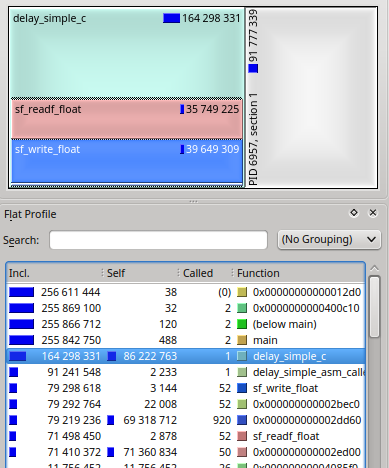
\includegraphics[scale=0.7]{imagenes/delay-overhead-libsndfile.png}
    \label{fig:delay-overhead-libsndfile}
    \caption{Delay libsndfile Overhead C}
\end{figure}

En la figura \ref{fig:delay-overhead-libsndfile}, la columna de la izquierda, con 3 filas, describe lo que pasa en el llamado a la función \textit{delay\_simple\_c}. Su costo total (164.000.000), está compuesto en un poco menos del 50\% ($35.000.000+40.000.000 = 75.000.000$) por los llamados a lectura y escritura de archivos.

\begin{figure}[H]
    \centering
    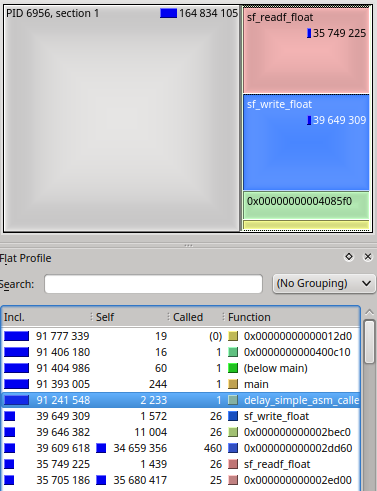
\includegraphics[scale=0.7]{imagenes/delay-overhead-libsndfile-asm.png}
    \label{fig:delay-overhead-libsndfile-asm}
    \caption{Delay libsndfile Overhead ASM}
\end{figure}

En la figura \ref{fig:delay-overhead-libsndfile-asm}, la columna de la derecha describe la función \textit{delay\_simple\_asm\_caller}; en este caso, la fila verde representa el código en el archivo \textbf{delay.asm}, y es notorio que su costo es muchísimo menor que los llamados a las funciones de la librería \textbf{libsndfile}, que son los que engrosan la cantidad total de instrucciones. 

\subsection{Análisis}


\newpage\section{Bibliografía tentativa}
\subsection{Libros}
\begin{thebibliography}{9}
 \bibitem{boulanger11}
  Richard Boulanger, Victor Lazzarini
  \emph{The Audio Programming Book},
  2011, The MIT Press, Massachussets (USA)
 
 \bibitem{moore90}
  F. Richard Moore,
  \emph{Elements of Computer Music},
  1990, Prentice Hall, New Jersey (USA)

  \bibitem{orfanidis10}
  Sophocles J. Orfanidis,
  \emph{Introduction to Signal Processing}, \\
  \url{http://www.ece.rutgers.edu/~orfanidi/intro2sp/}
  
  \bibitem{roads96}
  Curtis Roads,
  \emph{The Computer Music Tutorial},
  1996, The MIT Press, Massachussets (USA)
  \bibitem{rocchesso03}
  Davide Rocchesso,
  \emph{Introduction to Sound Processing},
  \url{profs.sci.univr.it/~rocchess/SP/sp.pdf}
  
  \bibitem{smith99}
  Steven W. Smith,
  \emph{The Scientist and Engineer's Guide to Digital Signal Processing},
  Second Edition, 1999, California Technical Publishing, California (USA)
  
  \bibitem{zolzer11}
  Udo Zölzer,
  \emph{DAFX: Digital Audio Effects}
  Second Edition, 2011, Wiley and Sons, Hamburg (Germany)
\end{thebibliography}
  
\subsection{Internet - links generales}
\begin{itemize}
\item \href{http://www.mega-nerd.com/libsndfile/api.html}{API de libsndfile}
\item \href{http://zetcode.com/gui/pyqt5/}{Ejemplos de uso de pyqt5}
\item \href{https://github.com/shuge/Qt-Python-Binding-Examples}{Más ejemplos de uso de pyqt5}
\item \href{https://ccrma.stanford.edu/~jos/}{Curso de Stanford: Introduction to Digital Filters}
\item \href{https://ccrma.stanford.edu/~jos/pasp/}{Curso de Stanford: Physical Audio Signal Processing}
\item \href{https://en.wikipedia.org/wiki/WAV}{Wikipedia: WAV file}
\item \href{https://en.wikipedia.org/wiki/Audio_signal}{Wikipedia: Audio signal}
\item \href{http://en.wikipedia.org/wiki/Sampling_rate}{Wikipedia: Sampling rate}
\item \href{https://en.wikipedia.org/wiki/Bit_rate}{Wikipedia: Bit rate}
\item \href{http://valgrind.org/docs/manual/cl-manual.html}{Valgrind: opciones para callgrind}
\item \href{http://kcachegrind.sourceforge.net/html/Tips.html}{KCacheGrind: profiling tips}
\item \href{http://whatis.techtarget.com/definition/flanging}{Definición flanging}
\item \href{http://www.h-schmidt.net/FloatConverter/IEEE754.html}{Conversor de números al formato IEEE754}
\item \href{http://www.cleavebooks.co.uk/scol/calnumba.htm}{Calculadora para cambio de base}
\item \url{http://stackoverflow.com}
\item \url{http://www.musicdsp.org/}
\item \url{http://www.kvraudio.org/}
\item \url{https://en.wikibooks.org/wiki/X86_Assembly/SSE}
\end{itemize}

\subsection{Fuentes de cosas específicas del TP}
\begin{itemize}
\item \underline{Figura \ref{fig:signals}}: \url{http://msp.ucsd.edu/techniques/v0.11/book-html/node7.html}
\item Ejemplo de uso de \fullref{subsec:libsndfile}: \url{http://www.labbookpages.co.uk/audio/wavFiles.html#c}
\item \underline{Algoritmo Delay}: variación de \href{http://stackoverflow.com/questions/5318989/reverb-algorithm}{Stack Overflow}, \href{http://www.musicdsp.org/showArchiveComment.php?ArchiveID=153}{MusicDSP}
\item \underline{Algoritmos Flanger, Vibrato y WahWah}: adaptación de \href{http://www.cs.cf.ac.uk/Dave/CM0268/Lecture_Examples/Digital_Audio_FX/flanger.m}{Cardiff School of Computer Science \& Informatics: MATLAB, DSP, Graphics CM0268}
\item \underline{Algoritmo Bitcrusher}: adaptación de \href{http://www.musicdsp.org/showArchiveComment.php?ArchiveID=139}{MusicDSP}

\end{itemize}

\end{document}
